\documentclass{epsrc}


%----These packages are only needed for drafts-----%
\usepackage{lipsum} % used for dummy text
\usepackage[colorinlistoftodos,prependcaption,textsize=tiny]{todonotes}%to do list and comments
\usepackage{soul}%highlighting etc
%--------------------------------------%


%I use these routinely but may not be needed
\usepackage{chemstyle}
\usepackage[version=3]{mhchem}
\usepackage{graphicx}
\usepackage{amsmath}
\usepackage{amsfonts}
\usepackage{hyperref}

%required for wrapping text around figures
\usepackage{wrapfig}

%set up different captions
\usepackage{caption}
\captionsetup[figure]{labelfont={it,bf},textfont=it}

%set up two bibliographies for parts 1 and 2
\usepackage[resetlabels]{multibib}
\newcites{A,B}{References,%
References}

\usepackage[british]{babel}

%%%Fancy header settings. Remove draft parts for final
\usepackage{fancyhdr}
\setlength{\headheight}{20pt}
\pagestyle{fancy}
\rhead[]{Prof. K. Benedek, et al}
\lhead[]{Mitigating Joule Expansion in Multicell Atomic Quantum Memory}
\chead[]{}
\rfoot[\textbf{Draft: \today}]{\textbf{Draft: \today}}%remove in final
\cfoot[\thepage]{\thepage}

\begin{document}
\section{Notes}
References cited with \verb|\citeA{}| will appear in the first bibliography. 
References cited with \verb|\citeB{}| will appear in the second bibliography (at the end).
You can \hl{highlight} or add comments \todo{like this} by using \verb|\hl{}| and \verb|\todo{}| respectively.
Comments will then be listed below.


\listoftodos%remove from final
\newpage% remove from final
\title{Mitigating Joule Expansion in Multicell Atomic Quantum Memory}
\author{Prof. K. Benedek, et al}
\maketitle

\section{Abstract}

The realisation of an effective method to read and write quantum information is of upmost importance to resolving current limitations in quantum communication systems \citeA{qRAMwalk}. Before scalable large-scale quantum networks can become a reality, various hardware design proposals for how to store communicated quantum information must be explored. Quantum computing and communication offer several advantages over the Classical Systems used today - namely, their superior computational ability in certain tasks grants the capability to break current data encryption algorithms \citeA{postQcrypto} and to offer greater computational disposal to future scientific research. Furthermore, they are unrivaled in their security of end-to-end information exchange \citeA{PubKeyQcrypto}. 

However, with the physical absence of scalable quantum information storage designs, the search for appropriate solutions continues. Herein, we propose to merge two existing technologies in order to improve the memory lifespan of Multicell Atomic Quantum Memory (MAQM) repeaters. By utilising optical tweezers to reduce the effects of atomic free expansion \citeA{OptTweezer}, dipole trap arrays can house microensembles of 2D atomic memory cell arrays and increase the memory lifespan of existing MAQM technology \citeA{MainMAQM} - our proposed method will increase the current state-of-the-art memory lifespan by up to three orders of magnitude. 

\part{Previous track record}

The Strathcylde Physics Department is a well-established and world-renowned centre for excellence in cold-atom systems and quantum algorithm development. The team selected for this proposal is no exception, and each bring their own strengths to this project, as listed below. Collaborators from M2Lasers will be offering specialised hardware for the experiment, expanding on their existing manufacturing expertise and product offerings. 

Furthermore, we are in collaboration with the primary researches from the Beijing Normal University who where responsible for the MAQM design, the prime set-up by which we will be basing our design from. Their results where published earlier in the year (2021), and their support will allow us to enchance the design and integrate their set-up with our proposed improvements.   \\

\section{EPSRC Relevance}

This proposal addresses the EPSRC Themes of ``Physical Sciences", ``Quantum Technologies", and ``Information and Communication Technologies". \\

\section{Contribution to UK Competitiveness}

\lipsum[75] \\

\section{Expertise at the Host Institution}

\textbf{Prof Kata Benedek} is..... \lipsum[66]

\textbf{Dr Christoforos Iacovou} is..... \lipsum[75]

\textbf{Dr Lewis MacLeod Russell} has completed previous EPSRC post-doctoral assistantships within the Department, after a successful PhD in ``Quantum Optics and Photonics" from the University. His expertise surrounding the Systems Integration of sensing apparatus with both optical and atomic dipole traps is directly transferable to the integration of the two proposed quantum technologies \citeA{OptTweezer, MainMAQM}. Dr. Russell participated in the design of similar quantum hardware in projects funded from EPSRC grants \href{https://gow.epsrc.ukri.org/NGBOViewGrant.aspx?GrantRef=EP/M013294/1}{EP/M013294/1}, \href{https://gow.epsrc.ukri.org/NGBOViewGrant.aspx?GrantRef=EP/T001046/1}{EP/T001046/1}, \href{https://gow.epsrc.ukri.org/NGBOViewGrant.aspx?GrantRef=EP/P009565/1}{EP/P009565/1}, and \href{https://gow.epsrc.ukri.org/NGBOViewGrant.aspx?GrantRef=EP/T005386/1}{EP/T005386/1}.    \\

\section{External Contributors}

Due to the successful research and subsequent publication regarding their MAQM experiment, Dr. Chang Li and
Dr. Yukai Wu of the Beijing Normal University will provide primary assistance in the replication of their hardware configuration - this then allows the Strathclyde team to adapt their configuration for our improved design with greater quantum memory lifetimes. Additionally, we call on the collaboration of Dr. Nils Hempler and his team from M2Lasers, based in Glasgow, to provide advanced laser systems hardware for our optical tweezers. Their existing capabilities in manufacturing advanced optical lattice hardware will be optimised for a new quantum system exclusively tailored for the loading of our atomic microensembles into our dipole trap array. \\

\bibliographystyleA{angew}
\bibliographyA{refs}

\newpage

\part{Description of proposed research and context}

\section{Vision, Aims and Context of the fellowship}

\lipsum[15-16]

\section{Adventure and potential impact}

\lipsum[17-18]

\begin{enumerate}[label=\roman*.]
	\item A
	\item B
	\item B
\end{enumerate}

\section{Research Concept}

\begin{figure}[!htbp]
	\begin{center}
		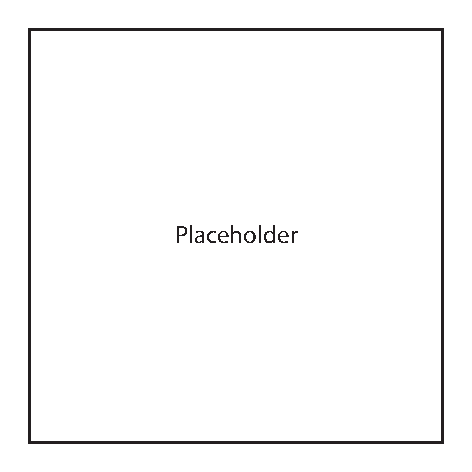
\includegraphics{img/placeholder_image}
		\vspace{-30pt}
		\caption{some caption}
		\label{fig:full}
	\end{center}
\end{figure}

\lipsum[19-20]

\begin{itemize}
	\item[-]A
	\item[-]B
	\item[-]C
\end{itemize}

\section{Background and Context}

\lipsum[21-22]

\begin{enumerate}[label=\bfseries \arabic*:, align=left]
	\item A
	\item B
	\item C
\end{enumerate}

\lipsum[23-24]

\begin{enumerate}[label=\bfseries Objective \arabic*:, align=left]
	\item A
	\item B
	\item B
	\item C
\end{enumerate}

\lipsum[25-26]

\begin{wrapfigure}{r}{0.5\textwidth}
\vspace{-11pt}
	\begin{center}
		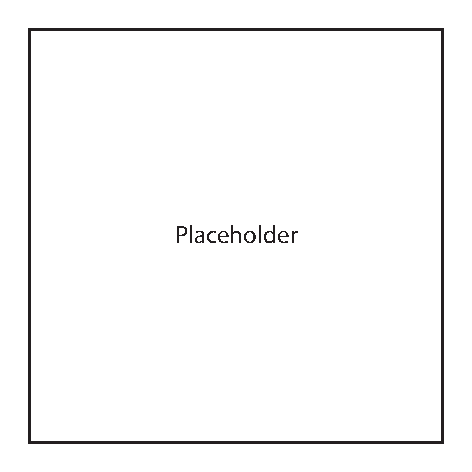
\includegraphics[width=8.5cm]{img/placeholder_image}
			\vspace{-30pt}
		\caption{A half width figure}
		\label{fig:half}
	\end{center}
\end{wrapfigure}

\lipsum[27-30]

\bibliographystyleB{angew}
\bibliographyB{refs} %your .bib file
\end{document}
